\documentclass{beamer}
%\usepackage{split}

\usepackage{amsmath}
\usepackage{amsfonts}
\usepackage{braket}
\usepackage{subcaption}
\usepackage{tikz}
\usepackage{xcolor}
%\usetikzlibrary{positioning,fit,backgrounds}
\usepackage{quantikz}
\usepackage[linesnumbered]{algorithm2e}
\usepackage{hyperref}
%\usepackage{hyperref,xcolor}
%\usepackage[ocgcolorlinks]{ocgx2}
\usepackage{cleveref}



\newcommand*{\QACze}{ \mathbf{QAC}_{0} }
\newcommand*{\QNCzef}{ \mathbf{QNC}_{0,f} }
\newcommand*{\QNCze}{ \mathbf{QNC}_{0} }
\newcommand*{\QNCon}{ \mathbf{QNC}_{1} }
\newcommand*{\NCon}{ \mathbf{NC}_{1} }
\newcommand*{\noiseQNCon}{ noisy-$\QNCon$ }
\newcommand*{\QNC}{ \mathbf{QNC} }
\newcommand*{\QNCG}{ \mathbf{QNC_G} }
\newcommand*{\NC}{\mathbf{NC}}
\newcommand*{\QNCiG}{\mathbf{QNC_{G,i}}}


\begin{document} 

\newcommand*{\Tr}{\textbf{Tr }}


\begin{frame}
  \title{Hardness of Computing Fault Tolerance.}
    \author{David Ponarovsky}
    \date{\today}
    \titlepage
\end{frame}


\begin{frame}

\frametitle{Introduction}
\begin{itemize}
    \item Brief overview of the topic
    \item Importance and relevance
    \item Objectives of the presentation
\end{itemize}
\end{frame}

\begin{frame}
\frametitle{Key Points}
\begin{itemize}
    \item Main point 1
    \item Main point 2
    \item Main point 3
\end{itemize}
\end{frame}


\begin{frame}{Definition}
%  \begin{block}{Definition}
\begin{definition}[$\NC$ - Nick's Class]
$\NC_i$ is the class of decision problems solvable by a uniform family of Boolean circuits, with polynomial size, depth $O(\log^i(n))$, and fan-in $2$. 
\end{definition}

\begin{definition}[$\QNC$]
  The class of decision problems solvable by polylogarithmic-depth, and finate fan out/in quantum circuits with bounded probability of error. Similarly to $\NC_i$, $\QNC_i$ is the class where the decisdes the circuits have $\log^i (n)$ depth.  
\end{definition}

\begin{definition}[$\QNCG$]
  For a fixing finate fan in/out gateset $G$, the class with deciding circuits composed only for gates in $G$ and at depath at most polylogaritmic. And in similar to $\QNC_{i}$, $\QNCiG$ is the restirction to circuits with depath at most $\log^{i}(n)$.  
\end{definition}
 % \end{block}
\end{frame}


\begin{frame}
  \frametitle{Nosiy Circuit.}

\begin{quantikz}[row sep=0.3cm, column sep=0.7cm]
\lstick{$q_1$} & \gate[wires=8]{U_0} & \gate{\mathcal{N}} & \gate[wires=8]{U_1}   & \gate{\mathcal{N}} & \gate[wires=8]{U_2} & \gate{\mathcal{N}}& \qw \\
\lstick{$q_2$} &                      & \gate{\mathcal{N}} &                      & \gate{\mathcal{N}} &                     & \gate{\mathcal{N}} & \qw \\
\lstick{$q_3$} &                      & \gate{\mathcal{N}} &                      & \gate{\mathcal{N}} &                     & \gate{\mathcal{N}} & \qw \\
\lstick{$q_4$} &                      & \gate{\mathcal{N}} &                      & \gate{\mathcal{N}} &                     & \gate{\mathcal{N}} & \qw \\
\lstick{$q_5$} &                      & \gate{\mathcal{N}} &                      & \gate{\mathcal{N}} &                     & \gate{\mathcal{N}} & \qw \\
\lstick{$q_6$} &                      & \gate{\mathcal{N}} &                      & \gate{\mathcal{N}} &                     & \gate{\mathcal{N}} & \qw \\
\lstick{$q_7$} &                      & \gate{\mathcal{N}} &                      & \gate{\mathcal{N}} &                     & \gate{\mathcal{N}} & \qw \\
\lstick{$q_8$} &                      & \gate{\mathcal{N}} &                      & \gate{\mathcal{N}} &                     & \gate{\mathcal{N}} & \qw
\end{quantikz}
\end{frame}

\begin{frame}{Nosiy Circuit.}
  \begin{definition}{ $p$- Depolarizing Channel. } 
    The qubit depolarizing channel with parameter $ p \in [0,1] $ is the quantum channel $ \mathcal{D}_p $ defined by:
\begin{equation*}
  \begin{split}
\mathcal{D}_p(\rho) = (1 - p) \rho + p \cdot \frac{I}{2}
  \end{split}
\end{equation*}

where $ \rho $ is a single-qubit density matrix and $ I $ is the identity matrix.

  \end{definition}
  \begin{definition}{$p$-Noisy Circuit.}
    Given a circuit $C$ (regardless of the model), its $p$-noisy version $\tilde{C}$ is the circuit obtained by alternately taking layers from $C$ and then passing each (qu)bit through a $p$-Depolarizing channel.
  \end{definition}
\end{frame}


\begin{frame}
  \frametitle{Threshoold Theorem.} 
\begin{center}
\begin{quantikz}[row sep=0.3cm, column sep=0.4cm]
\lstick[2]{$\ket{\psi}_L$} & \gate[2,style={fill=red!20}]{U_L} & \qw & \qw \\
                          &                                   &     &     \\
\lstick{$\ket{\psi_1}$}   & \gate[5,style={fill=blue!10}]{\text{Gadget for } U_L} & \qw & \qw \\
\lstick{$\ket{\psi_2}$}   &                                                                 & \qw & \qw \\
\lstick{$\ket{\psi_3}$}   &                                                                 & \qw & \qw \\
\lstick{$\ket{\psi_4}$}   &                                                                 & \qw & \qw \\
\lstick{$\ket{\psi_5}$}   &                                                                 & \qw & \qw \\
\end{quantikz}
\end{center}

\end{frame}



\begin{frame}
  \frametitle{Pippenger's Construction.} 
  
Encode each bit with the repetition code $0 \mapsto 0^{m}$, $1 \mapsto 1^{m}$. Now observe that any logical operation, without decoding, can be made in $O(1)$ depth.

For example, OR($\bar{x}, \bar{y}$) can be computed by applying in parallel OR($x_{i}, y_{i}$) for each $i$.

\end{frame}


\begin{frame}
  \frametitle{The 'Decoding' trick.} 

Instead of completely decoding, we would apply only a single step of partial decoding. We assume that in each code block the bits are partitioned into random disjoint triples, and we will apply a local correction to each of the triples by majority.



\begin{block}{Claim}
There are constants $\alpha, \eta \in (0,1)$ such that for any bit string $x$ at a distance $\le \alpha n$ from the code (Repetition Code), one cycle of local correction on $x$ yields $x^\prime$ such that:
  \begin{equation*}
    \begin{split}
      d(x^{\prime}, C) \le d(x, C)
    \end{split}
  \end{equation*}
\end{block}
\end{frame}


\begin{frame}
  \frametitle{The 'Decoding' trick.} 
  
  Suppose that a bit obserb a bit flip with probability $p$. So in expectation we expect that entire bolck at length $n$ will absorb $pn$ flips.  
  \begin{equation*}
    \begin{split}
      \eta \left( \beta + p  \right) n &\le \beta n \\ 
      \beta \ge \frac{p}{ 1 - \eta}
    \end{split}
  \end{equation*}


\end{frame}

\begin{frame}

  From now on, we will assume that the graphs are bipartite and we will denote the right and the left vertices by $V^{-}$ and $V^{+}$. Notice that such expanders near Ramanujan exist, see for example \cite{leverrier2022decodingquantumtannercodes}. The partition into two subsets enable us to come with a simple efficient decoder.

  Expanders code are known for having good decoders, beneath, in \Cref{alg:three}, we introduce a procedure to reduce an error. In overall, we alternately let to the right and then the left vertices to correct their own local view. In \Cref{lemma:reduce} we prove that when the applied error has size at most $\beta n$, for some constant $\beta$ then the error's weight reduced by $\frac{1}{2}$. Repeating over the procedure $\Theta(\log(n) )$ times completely correct the error. 

\end{frame}
\begin{frame}

  We will call to the first stage, when only the right vertices suggest correction the right round, and to the second stage a left round. For the whole procedure, we will call a single correction round.  

  
  \begin{figure}[h]
    \begin{subfigure}[h]{0.05\textwidth}
      \
    \end{subfigure}
    \begin{subfigure}[h]{0.40\textwidth}

    \label{alg:three}
      \begin{algorithm}[H]
    \caption{Single decoding round}
    \KwData{ $x \in \mathbb{F}_{2}^{n}$ }
    \KwResult{ $\arg\min {\left\{  y \in C : |y + x|  \right\} }$ if $d(y,C) <$ }
    \For { $ v \in V^{+}$} {
      $x^{\prime}_{v} \leftarrow \arg\min {\left\{  y \in C_{0} : |y + x|_{v} |  \right\} } $\\
    }
    \For { $ v \in V^{-}$} {
      $x^{\prime}_{v} \leftarrow \arg\min {\left\{  y \in C_{0} : |y + x|_{v} |  \right\} } $\\
    }
    \Return  $x $

  \end{algorithm}
    \end{subfigure}
    \begin{subfigure}[h]{0.05\textwidth}
      \
    \end{subfigure}
    \begin{subfigure}[h]{0.40\textwidth} 

    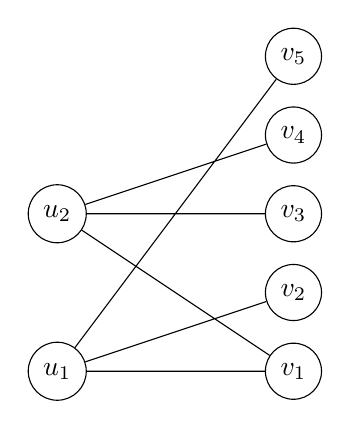
\begin{tikzpicture}%[scale=2.5]
\tikzstyle{every node}=[draw,shape=circle];

\draw node (v0) at (0,1) {$u_1$};
\draw node (v6) at (0,3) {$u_2$};
\draw node foreach \x in {1,2,3,4,5} (v\x) at (3,\x) {$v_\x$};

%\path (0:0cm) node (v0) {$v_0$};
%\path (-36:1cm) node (v1) {$v_1$};
%\path (-2*36:1cm) node (v2) {$v_2$};
%\path (0:1cm) node (v3) {$v_3$};
%\path (36:1cm) node (v4) {$v_4$};
%\path (2*36:1cm) node (v5) {$v_5$};
\draw (v0) -- (v1)
(v0) -- (v2)
(v0) -- (v5)
(v6) -- (v3)
(v6) -- (v4)
(v6) -- (v1);
\end{tikzpicture}
\caption{location.}
    \label{fig:location}
    \end{subfigure} 
  \end{figure}
  \begin{lemma}
    \label{lemma:reduce}
    If the error is at wight less than $\beta n $ then a single round of the  majority reduce the error by at least constant fraction. 
  \end{lemma}

\end{frame}
\begin{frame}

  Denote by $S^{(0)} \subset V^{+}$ and  $T^{(0)} \subset V^{-}$ the subsets of left and right vertices adjacent to the error. And denote by $T^{(1)} \subset T^{(0)}$ the right vertices such any of them is connect by at least $\frac{1}{2}\delta_{0}\Delta$ edges to vertices at $S^{(0))}$. Note that that any vertex in $V^{-}/T^{(1)}$ has on his local view less than $\frac{1}{2}\delta_{0}\Delta$ faulty bits, So it corrects into his right local view in the first right correction round. Therefore after the right correction round the error is set only on $T^{(1)}$'s neighbourhood, namely at size at most $\Delta|T^{(1)}|$.  We will show that this amount is strictly lower by a constant factor than $|e|$. 

\end{frame}
\begin{frame}

  First, let's use the expansion property (\Cref{def:mix}) for getting an upper bound on $T^{(1)}$ size: \begin{equation*}
  \begin{split} 
    \frac{1}{2}\delta_{0}\Delta |T^{(1)}| & \le \Delta \frac{|T^{(1)}||S^{(0)}|}{n} + \lambda\sqrt{|T^{(1)}||S^{(0)}|} \\ 
  \left( \frac{1}{2} \delta_{0} \Delta - \frac{|S^{(0)}|}{n} \Delta \right) |T^{(1)}| & \le \lambda \sqrt{|T^{(1)}||S^{(0)}|} \\ 
|T^{(1)}| & \le \left( \frac{1}{2} \delta_{0} \Delta - \frac{|S^{(0)}|}{n} \Delta \right)^{-2}\lambda^{2} |S^{(0)}| 
  \end{split}
\end{equation*}
Since any left vertex adjoins to at most $\Delta$ faulty bits we have that $\Delta|S^{(0)}| \le |e|$. Combing with the inequality above we get:  

\begin{equation*}
  \begin{split}
    \Delta |T^{(1)}| \le \left( \frac{1}{2} \delta_{0} \Delta - \frac{|e|}{n} \right)^{-2}\lambda^{2} |e|
  \end{split}
\end{equation*}
Hence for $|e|/n \le \beta =  \frac{1}{2} \delta_{0} \Delta - \sqrt{2\lambda}$ it holds that $\Delta|T^{(1)}| \le \frac{1}{2}|e|$. Namely the error is reduced by half.  




\end{frame}




\begin{frame}
  \frametitle{The Franch's Construction.}
\end{frame}


\begin{frame}
  \frametitle{  }


\begin{figure}[h]
    \centering
    \includegraphics[width=\textwidth]{Hypergraph_prod.png}
    \caption{Caption for the image}
    \label{fig:your-label}
\end{figure}

\end{frame}

\begin{frame}
  \frametitle{  }

\begin{figure}[h]
    \centering
    \includegraphics[width=0.8\textwidth]{toric_prod.png}
    \caption{Caption for the image}
    \label{fig:your-label}
\end{figure}

\end{frame}
\begin{frame}
  \frametitle{ } 
\begin{figure}[h]
    \centering
    \includegraphics[width=\textwidth]{magic_prod.png}
    \caption{Caption for the image}
    \label{fig:your-label}
\end{figure}
\end{frame}



\begin{frame}
  \frametitle{Disjointness.}
\end{frame}

\end{document}
